\begin{wrapfigure}{r}{9cm}
  \centering
  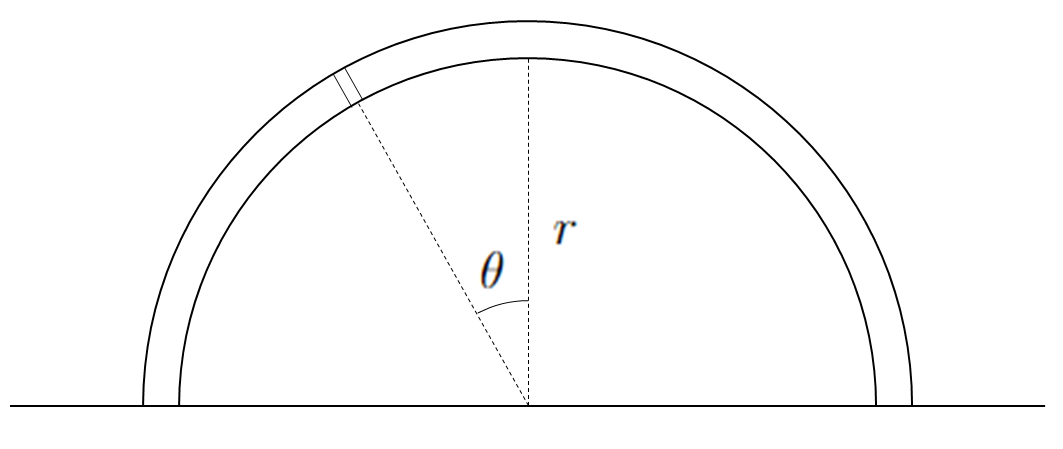
\includegraphics[width=0.5\textwidth]{images/Hinh 2.PNG}
  \vspace{-25px}
  \begin{center}
    \figurename{ 2}
  \end{center}
  \vspace{15px}
\end{wrapfigure}

\vspace{-30px}
\noindent Một ống thuỷ tinh mỏng, tiết diện đều, hai đầu bịt kín được uốn thành một nửa đường tròn bán kính $r$ (bán kính tiết diện của ống rất nhỏ so với $r$) sau đó được gắn cố định trên trên mặt sàn nằm ngang sao cho toàn bộ ống nằm trong mặt phẳng thẳng đứng như hình 2. Bên trong ống có một piston mỏng có khối lượng $m$ được làm bằng kim loại, diện tích của piston bằng với tiết diện của ống thuỷ tinh. Đường nối tâm đường tròn và vị trí của piston hợp với phương thẳng đứng một góc $\theta$. Hai bên piston đều chứa n mol khí lý tưởng, giả sử nhiệt độ của khí luôn bằng nhiệt độ $T$ của môi trường bên ngoài. Cho biết gia tốc trọng trường có độ lớn $g$, hằng số khí lý tưởng $R$, xem như tất cả các quá trình biến đổi trạng thái của khí đều chuẩn tĩnh. Bỏ qua mọi ma sát.\\
\vspace{-15pt}
\begin{enumerate}
  \item Khi nhiệt độ $T$ lớn hơn một nhiệt độ tới hạn $T_{C}$ nào đó, vị trí cân bằng bền của piston nằm ngay chính giữa ống ($\theta=0$). Hãy tìm biểu thức của $T_{C}$ và xác định tần số góc trong dao động bé của piston quanh vị trí cân bằng này.
  \item Khi $T=T_{C}$, hãy đánh giá tính ổn định của piston khi nó nằm cân bằng ở giữa ống ($\theta=0$).\\
\end{enumerate}
\vspace{-15px}
\noindent Đối với các câu hỏi bên dưới, xem $T_{C}$ như một thông số đã biết và không cần thay vào giá trị mà bạn đã tìm được ở ý 1.
\begin{enumerate}
  \setcounter{enumi}{2}
  \item Khi $T<T_{C}$, piston cân bằng tại vị trí góc $\theta_{0}$, tìm phương trình mà $\theta_{0}$ phải thoả mãn. Xác định biểu thức gần đúng khi nhiệt độ $T$ giảm nhẹ (xấp xỉ đến bậc thấp nhất khác 0).
  \item Khi $T<T_{C}$, xác định tần số góc $\omega_{0}$ trong dao động bé của piston quanh vị trí cân bằng tại $\theta_{0}$, tần số này bằng bao nhiêu khi nhiệt độ của khí lớn hơn và nhỏ hơn $T_{C}$ một chút.
  \item Khi $T<T_{C}$, giả sử vận tốc ban đầu của piston gần như bằng không, hãy tìm độ lớn vận tốc góc của piston khi nó di chuyển từ vị trí chính giữa $(\theta=0)$ đến vị trí góc lớn nhất $\theta$ mà nó có thể đi được.
\end{enumerate}